\section{Results}\label{sec:results}

\subsection{Climate and model behaviour}
Fig.~\ref{fig:climate} summarises the ISHRAE typical year. Mean monthly dry-bulb
temperature peaks at 29.1\,$^\circ$C in May, and the hourly maximum of 41.0\,$^\circ$C
falls in the extreme week of 6--12~May. Monsoon humidity exceeds 80\,\% from July to
October. The roof slab and walls make the house slow to respond: the mass time constants
are 25--36\,h, while the air nodes respond within about 25\,min. Fig.~\ref{fig:week}
shows the behaviour of each controller during the extreme week.
\begin{itemize}
  \item The thermostat cycles each indoor unit on and off at full capacity, roughly
        every 15--30\,min, producing a 1--2\,K sawtooth.
  \item PID holds each zone close to the 24.5\,$^\circ$C setpoint.
  \item E-MPC and Hybrid keep occupied zones just inside the 26\,$^\circ$C upper bound
        (minus the 0.5\,K back-off), which is the cheapest admissible temperature.
\end{itemize}

\begin{figure}[t]\centering
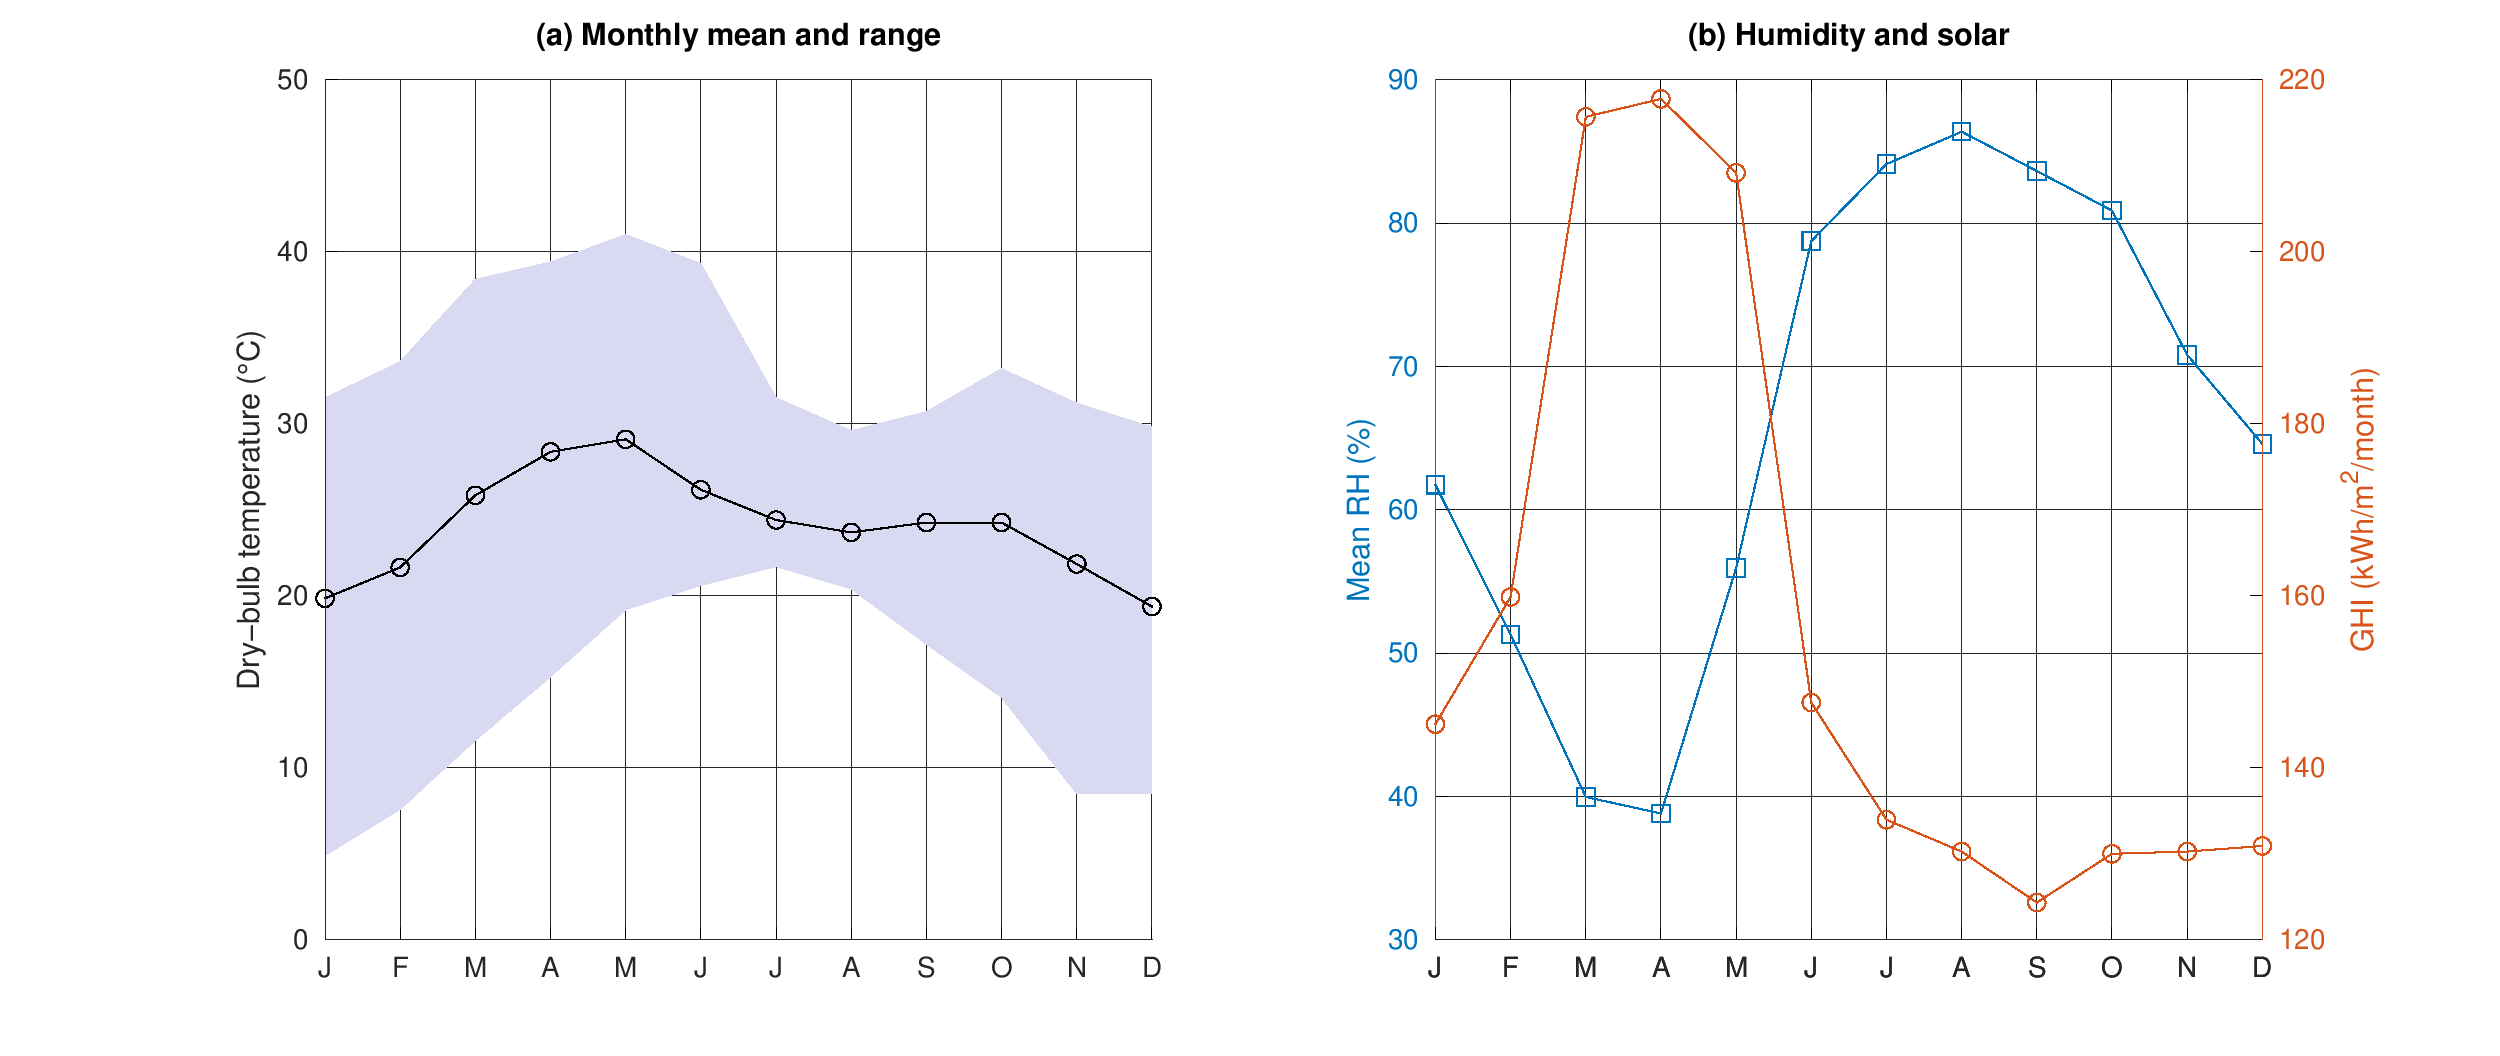
\includegraphics[width=\linewidth]{Fig01_climate.png}
\caption{ISHRAE typical-year climate for Pune: (a) monthly mean and range of dry-bulb
temperature; (b) mean relative humidity and monthly global horizontal irradiation.}
\label{fig:climate}
\end{figure}

\begin{figure}[t]\centering
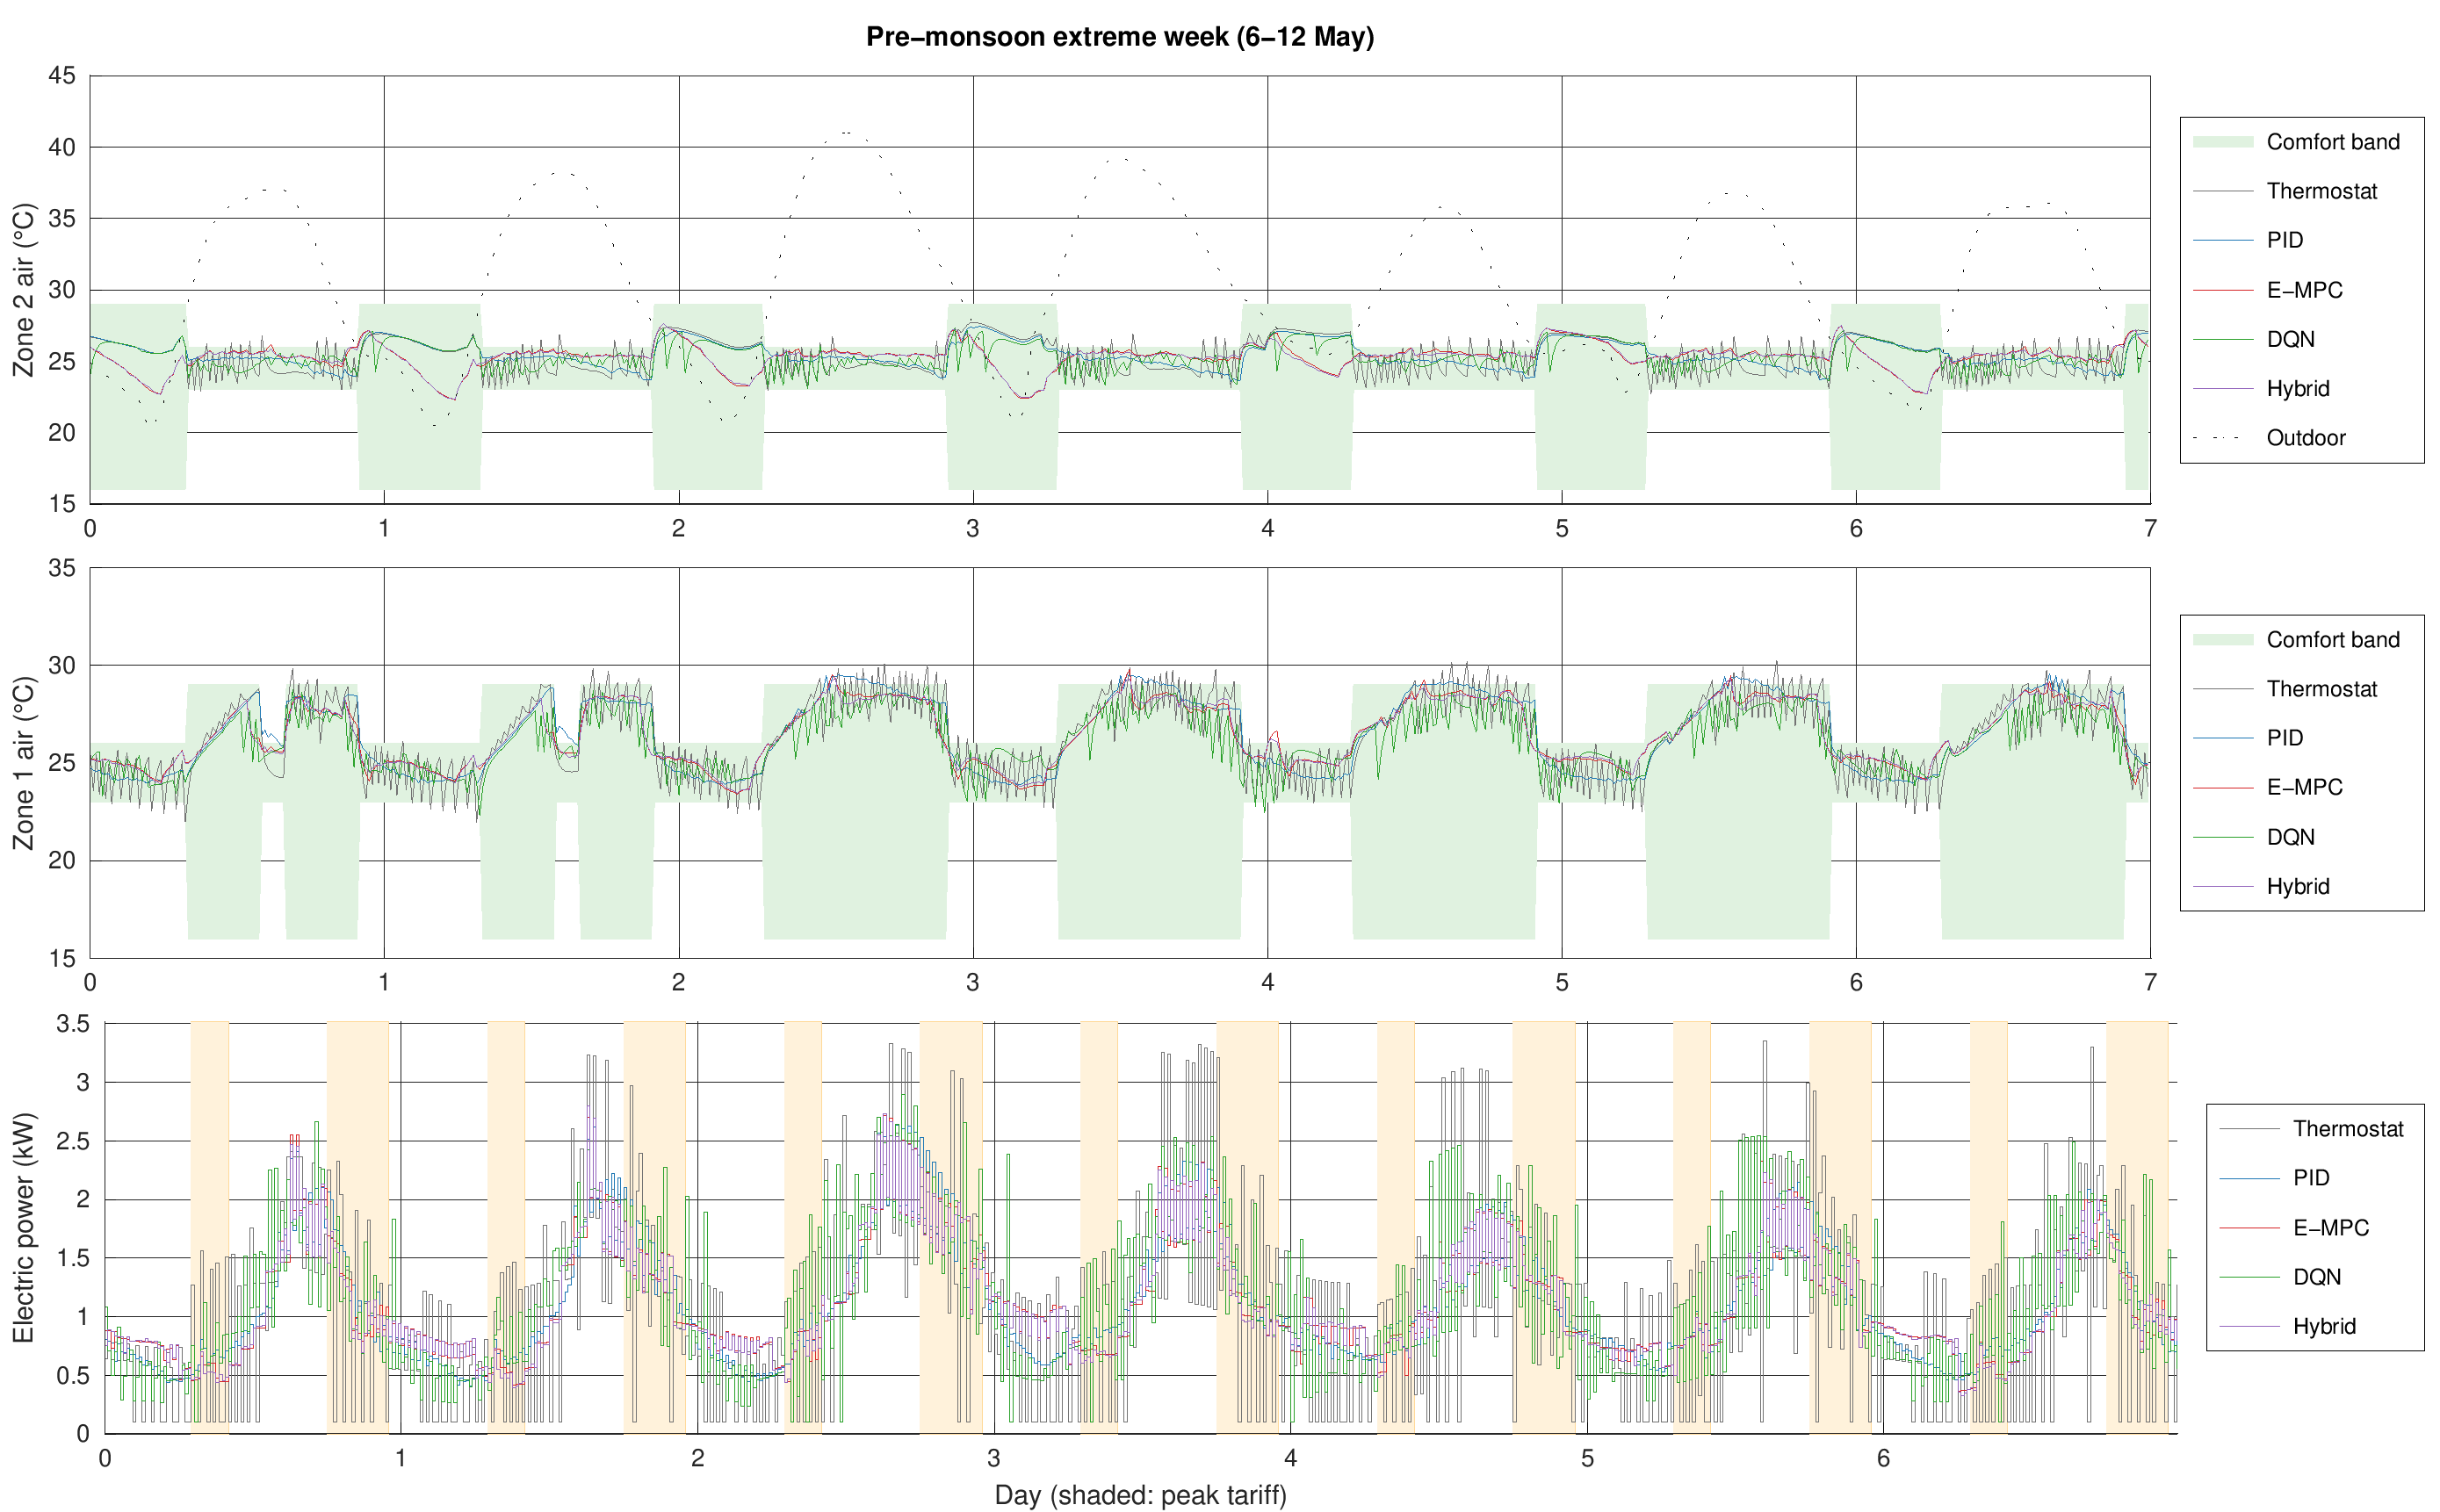
\includegraphics[width=\linewidth]{Fig02a_week_1.png}
\caption{Extreme pre-monsoon week (6--12 May), seed 1. Top: Zone~2 air temperature with
the occupancy-dependent comfort band (shaded) and outdoor temperature. Middle: Zone~1.
Bottom: total electric power, with peak-tariff hours shaded.}
\label{fig:week}
\end{figure}

\subsection{Annual cost, energy and comfort}
Table~\ref{tab:main} and Fig.~\ref{fig:pareto} give the annual results, as the mean
and 95\,\% interval over five seeds.

\textbf{Thermostat: cheapest, but at the cost of comfort.} The thermostat has the
lowest electricity cost (INR~\CostTh) and energy use (\ETh\,kWh). It also has the
largest discomfort (\KhTh\,K\,h) and the lowest share of acceptable occupied zone-hours
(\AccTh\,\%). Most of that discomfort is cooling-induced overcooling (\KhColdTh\,K\,h):
each unit runs at full capacity until the zone is 0.5\,K below the setpoint, and the
air node's 25-min time constant carries it well below 23\,$^\circ$C. The thermostat
also starts the compressor about \StartsRatioTh{} times more often than the Hybrid
controller.

\textbf{The four modulating controllers.} All four cut discomfort by 71--83\,\%
compared with the thermostat, and they spend 3--7\,\% more on electricity to do it.
\begin{itemize}
  \item \textbf{Hybrid} has the lowest discomfort (\KhHyb\,K\,h, \AccHyb\,\% acceptable)
        and is the cheapest of the four (INR~\CostHyb). Against PID it reduces cost by
        \RelHybPidCost\,\% and discomfort by \RelHybPidKh\,\%. Against E-MPC it reduces
        cost by \RelHybMpcCost\,\% and discomfort by \RelHybMpcKh\,\%.
  \item \textbf{E-MPC} costs \RelMpcPidCost\,\% less than PID, with discomfort that is
        \RelMpcPidKh\,\% lower (\KhMpc\ vs \KhPid\,K\,h).
  \item \textbf{DQN} (shielded) lies between PID and E-MPC on cost (INR~\CostDqn) and
        matches E-MPC on discomfort (\KhDqn\,K\,h). It is the only controller whose
        outcome varies materially between seeds (cost $\pm$\CostDqnCI, discomfort
        $\pm$\KhDqnCI), reflecting differences between training runs.
\end{itemize}
The seed intervals of the other controllers are narrow: sensor noise and forecast
errors change annual cost by less than 0.1\,\%.

\begin{table}[t]\centering\small
\caption{Annual results, mean $\pm$ 95\,\% CI over five seeds. Discomfort counts
occupied overheating plus cooling-induced overcooling (K\,h); "acceptable" is the
share of occupied zone-hours without either. $\Delta$cost is relative to the
thermostat.}\label{tab:main}
% generated by aggregate_results.m -- mean +/- 95% CI over 5 seeds
\begin{tabular}{lrrrrrrr}
\hline
Controller & Energy (kWh) & Cost (INR) & $\Delta$cost & Discomfort (K\,h) & Acceptable (\%) & RMSE (K) & Peak (kW)\\
\hline
Thermostat & 5028 $\pm$ 1 & 36950 $\pm$ 8 & -- & 1101.5 $\pm$ 3.2 & 82.7 $\pm$ 0.1 & 1.17 $\pm$ 0.00 & 3.38 $\pm$ 0.01\\
PID & 5403 $\pm$ 0 & 39460 $\pm$ 3 & +6.8\% & 315.3 $\pm$ 0.5 & 94.8 $\pm$ 0.0 & 0.75 $\pm$ 0.00 & 2.69 $\pm$ 0.04\\
E-MPC & 5243 $\pm$ 3 & 38306 $\pm$ 26 & +3.7\% & 250.6 $\pm$ 2.2 & 95.7 $\pm$ 0.0 & 0.99 $\pm$ 0.00 & 2.78 $\pm$ 0.07\\
DQN & 5273 $\pm$ 112 & 38799 $\pm$ 682 & +5.0\% & 259.2 $\pm$ 53.8 & 94.3 $\pm$ 0.8 & 0.90 $\pm$ 0.04 & 3.32 $\pm$ 0.07\\
Hybrid & 5198 $\pm$ 1 & 38005 $\pm$ 14 & +2.9\% & 185.1 $\pm$ 1.1 & 96.1 $\pm$ 0.0 & 0.99 $\pm$ 0.00 & 2.78 $\pm$ 0.10\\
\hline
\end{tabular}

\end{table}

\begin{figure}[t]\centering
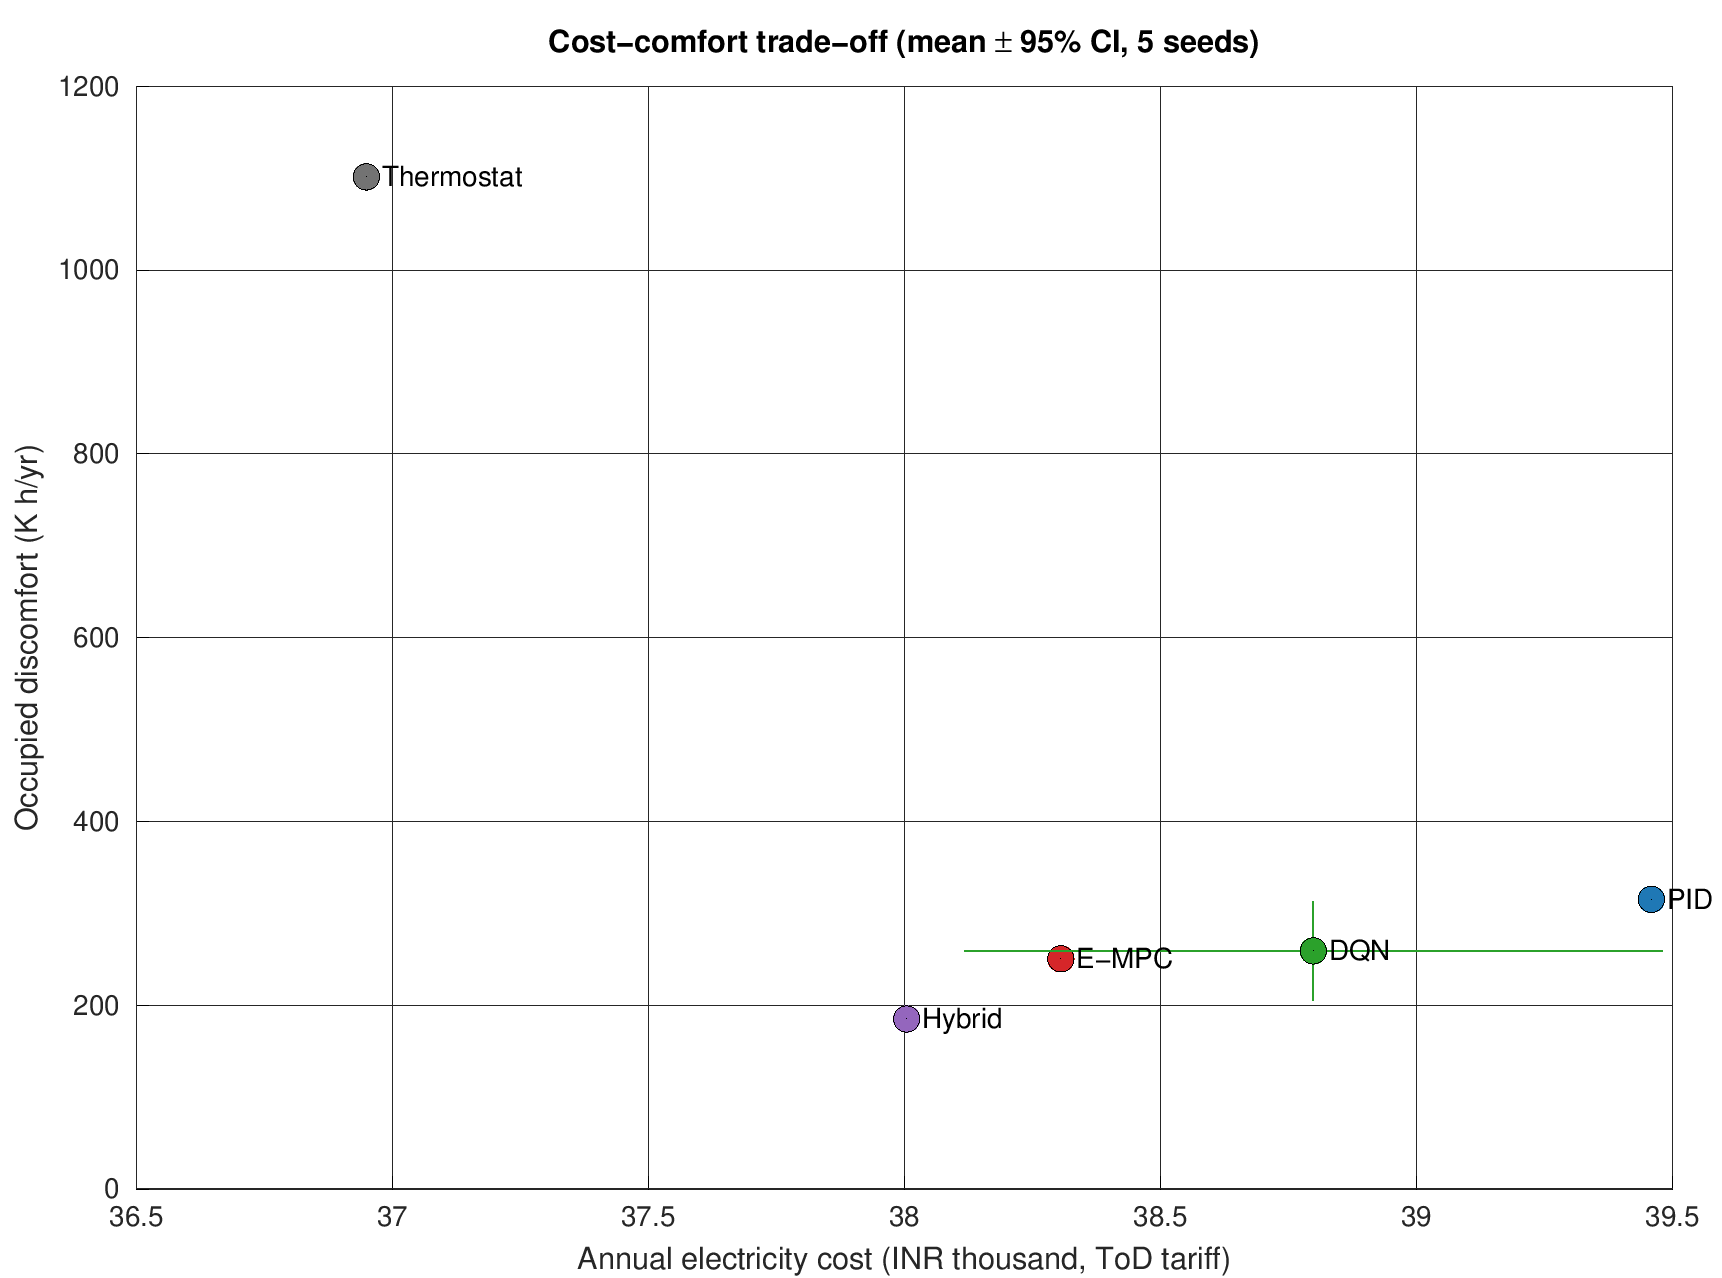
\includegraphics[width=0.62\linewidth]{Fig05_pareto.png}
\caption{Annual ToD electricity cost versus occupied discomfort (mean $\pm$ 95\,\% CI over
five seeds).}\label{fig:pareto}
\end{figure}

\paragraph{Paired daily comparisons.}
These use seed~1 with a block bootstrap and the Wilcoxon signed-rank test.
\begin{itemize}
  \item Hybrid vs PID: cost INR~$\PairHybridPidCost${}
        [$\PairHybridPidCostLo$, $\PairHybridPidCostHi$], $p\PairHybridPidCostP$; discomfort
        $\PairHybridPidKh$\,K\,h [$\PairHybridPidKhLo$, $\PairHybridPidKhHi$],
        $p\PairHybridPidKhP$. Both differences are significant.
  \item Hybrid vs E-MPC: cost INR~$\PairHybridMpcCost${}
        [$\PairHybridMpcCostLo$, $\PairHybridMpcCostHi$]; discomfort $\PairHybridMpcKh$\,K\,h
        [$\PairHybridMpcKhLo$, $\PairHybridMpcKhHi$]; both $p\PairHybridMpcCostP$. Both
        differences are significant.
  \item E-MPC vs PID: the discomfort difference is not significant
        ($p=\PairMpcPidKhP$), but the cost saving is
        (INR~$\PairMpcPidCost${} [$\PairMpcPidCostLo$, $\PairMpcPidCostHi$]).
\end{itemize}

\subsection{Where the energy goes}
Fig.~\ref{fig:energy} breaks electricity down by month and end use.
\begin{itemize}
  \item The VRF accounts for 61--65\,\% of annual electricity.
  \item The DOAS (fans, energy recovery and the demand-controlled dehumidifying coil)
        uses 1.2--1.3\,MWh, about a quarter of the total, mostly during the monsoon. It
        is the largest load outside the controllers' authority.
  \item The recirculation filter fan adds a constant 0.53\,MWh.
  \item The IEC uses 0.1--0.2\,MWh and runs for 580--1100\,h in the dry pre-monsoon.
        Its runtime depends on the controller, because it is enabled only while
        cooling is requested.
\end{itemize}
Monthly electricity peaks in May at 760--805\,kWh and is lowest in December and January.

\begin{figure}[t]\centering
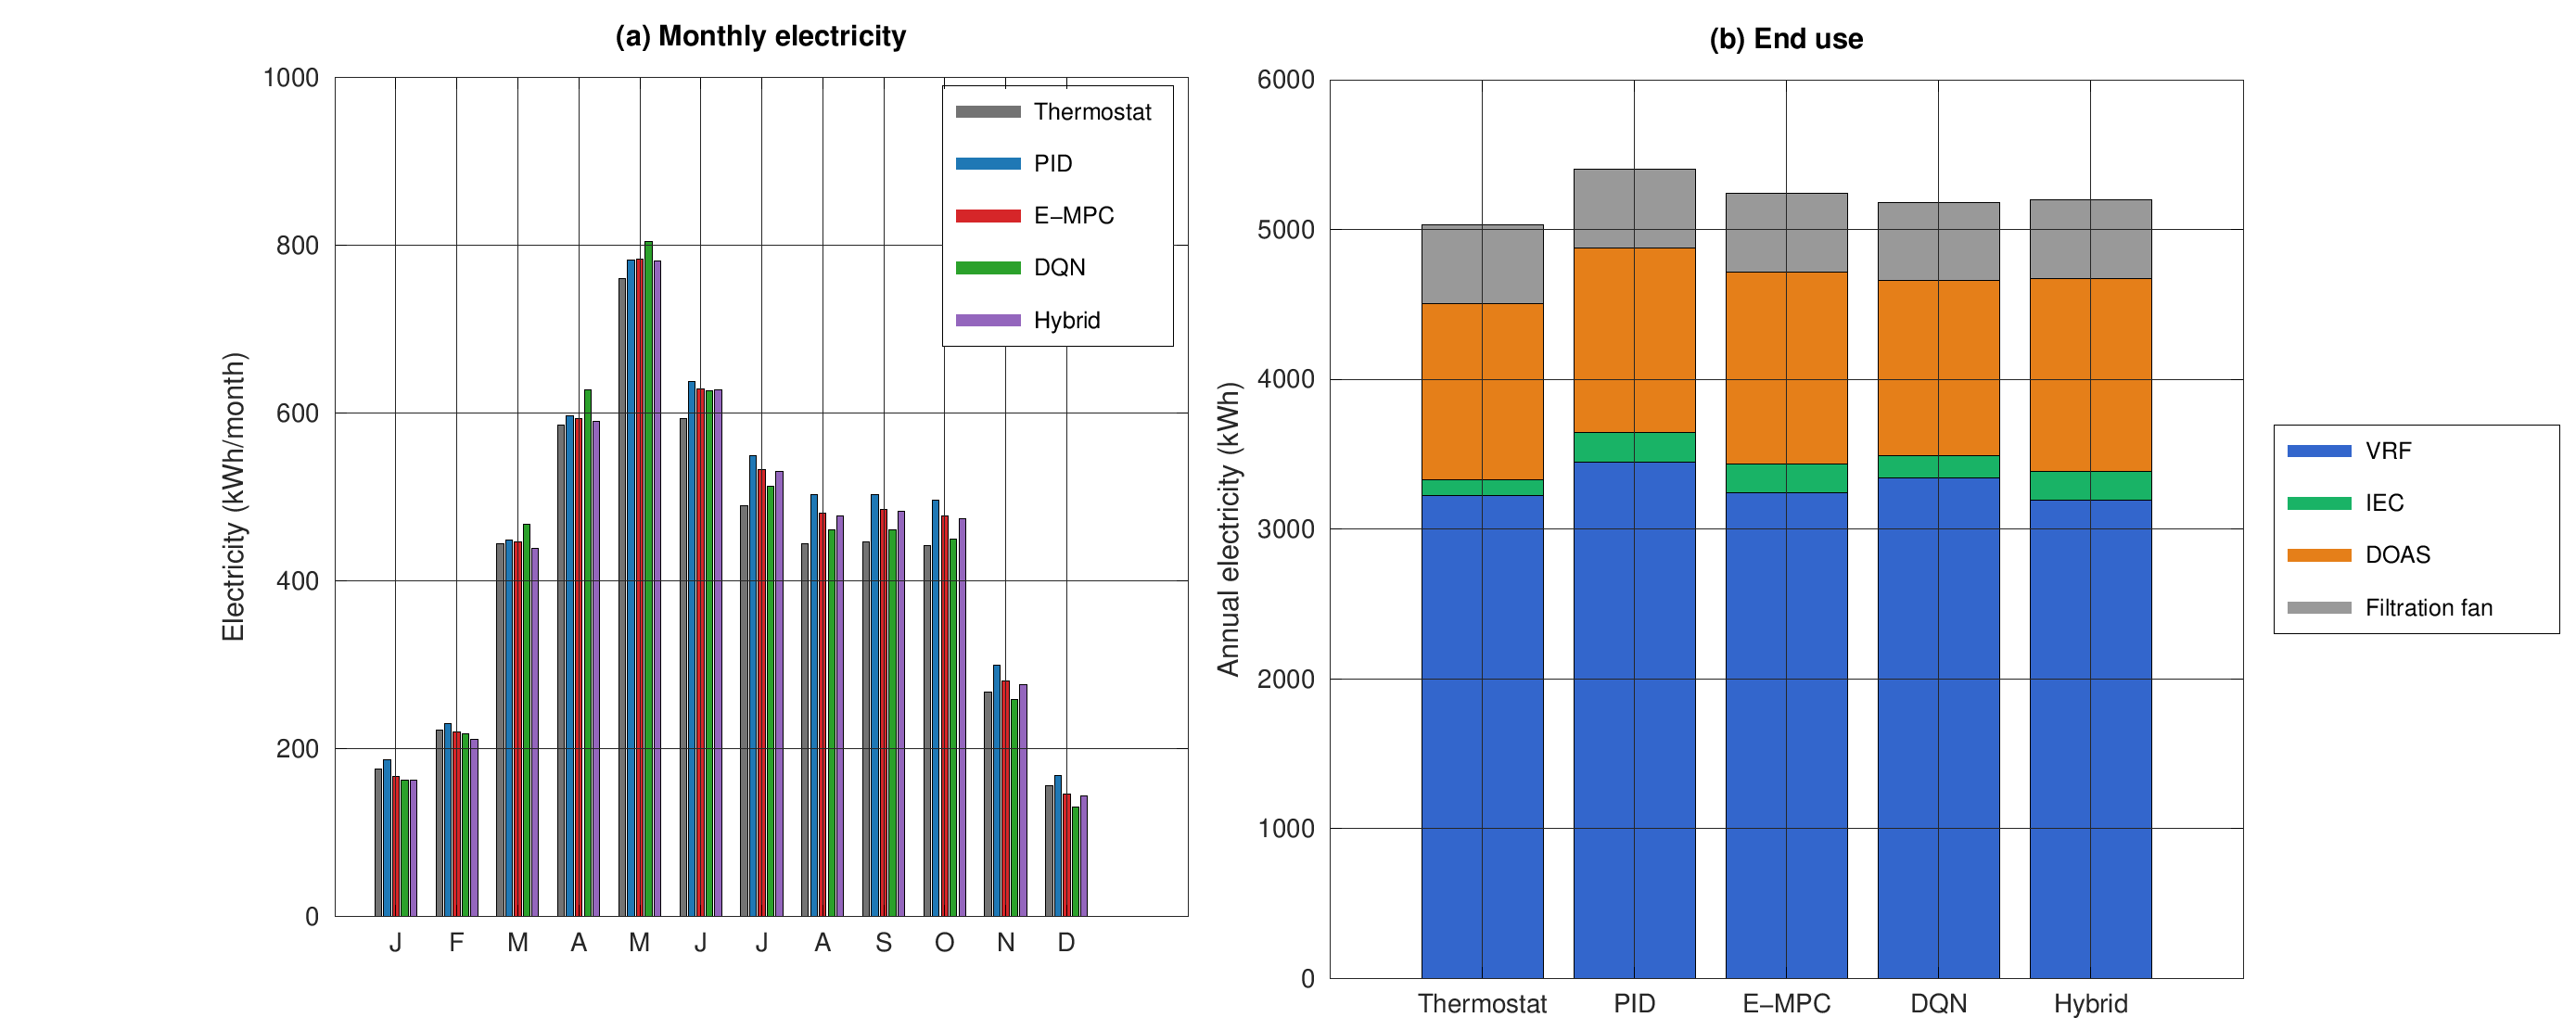
\includegraphics[width=\linewidth]{Fig03_energy.png}
\caption{(a) Monthly electricity (actual monthly sums) and (b) annual end-use split, seed 1.}
\label{fig:energy}
\end{figure}

\subsection{Load shifting under the ToD tariff}
Fig.~\ref{fig:profile} shows the mean daily profile of VRF power for March to June.
E-MPC and Hybrid draw more power than PID between 00:00 and 05:00, when the tariff is
off-peak, and less around 10:00--11:00, so they pre-cool the thermal mass at night.
The share of VRF energy used in peak-tariff hours, however, is almost the same for every
controller (\PeakShareTh--\PeakShareDqn\,\%). The flat-tariff scenario confirms this:
removing the ToD signal changes E-MPC energy use by less than 0.5\,\%
(Section~\ref{sec:sens}). The economic MPC's advantage therefore comes mainly from
temperature-aware efficiency (cooling when the COP is higher) and from riding the upper
comfort bound. It does not come from moving demand out of the 07:00--10:00 and
18:00--23:00 peak windows: all peak-window cooling serves occupied zones, and the
day's stored heat is released from the slab in the evening (Section~\ref{sec:discussion}).

\begin{figure}[t]\centering
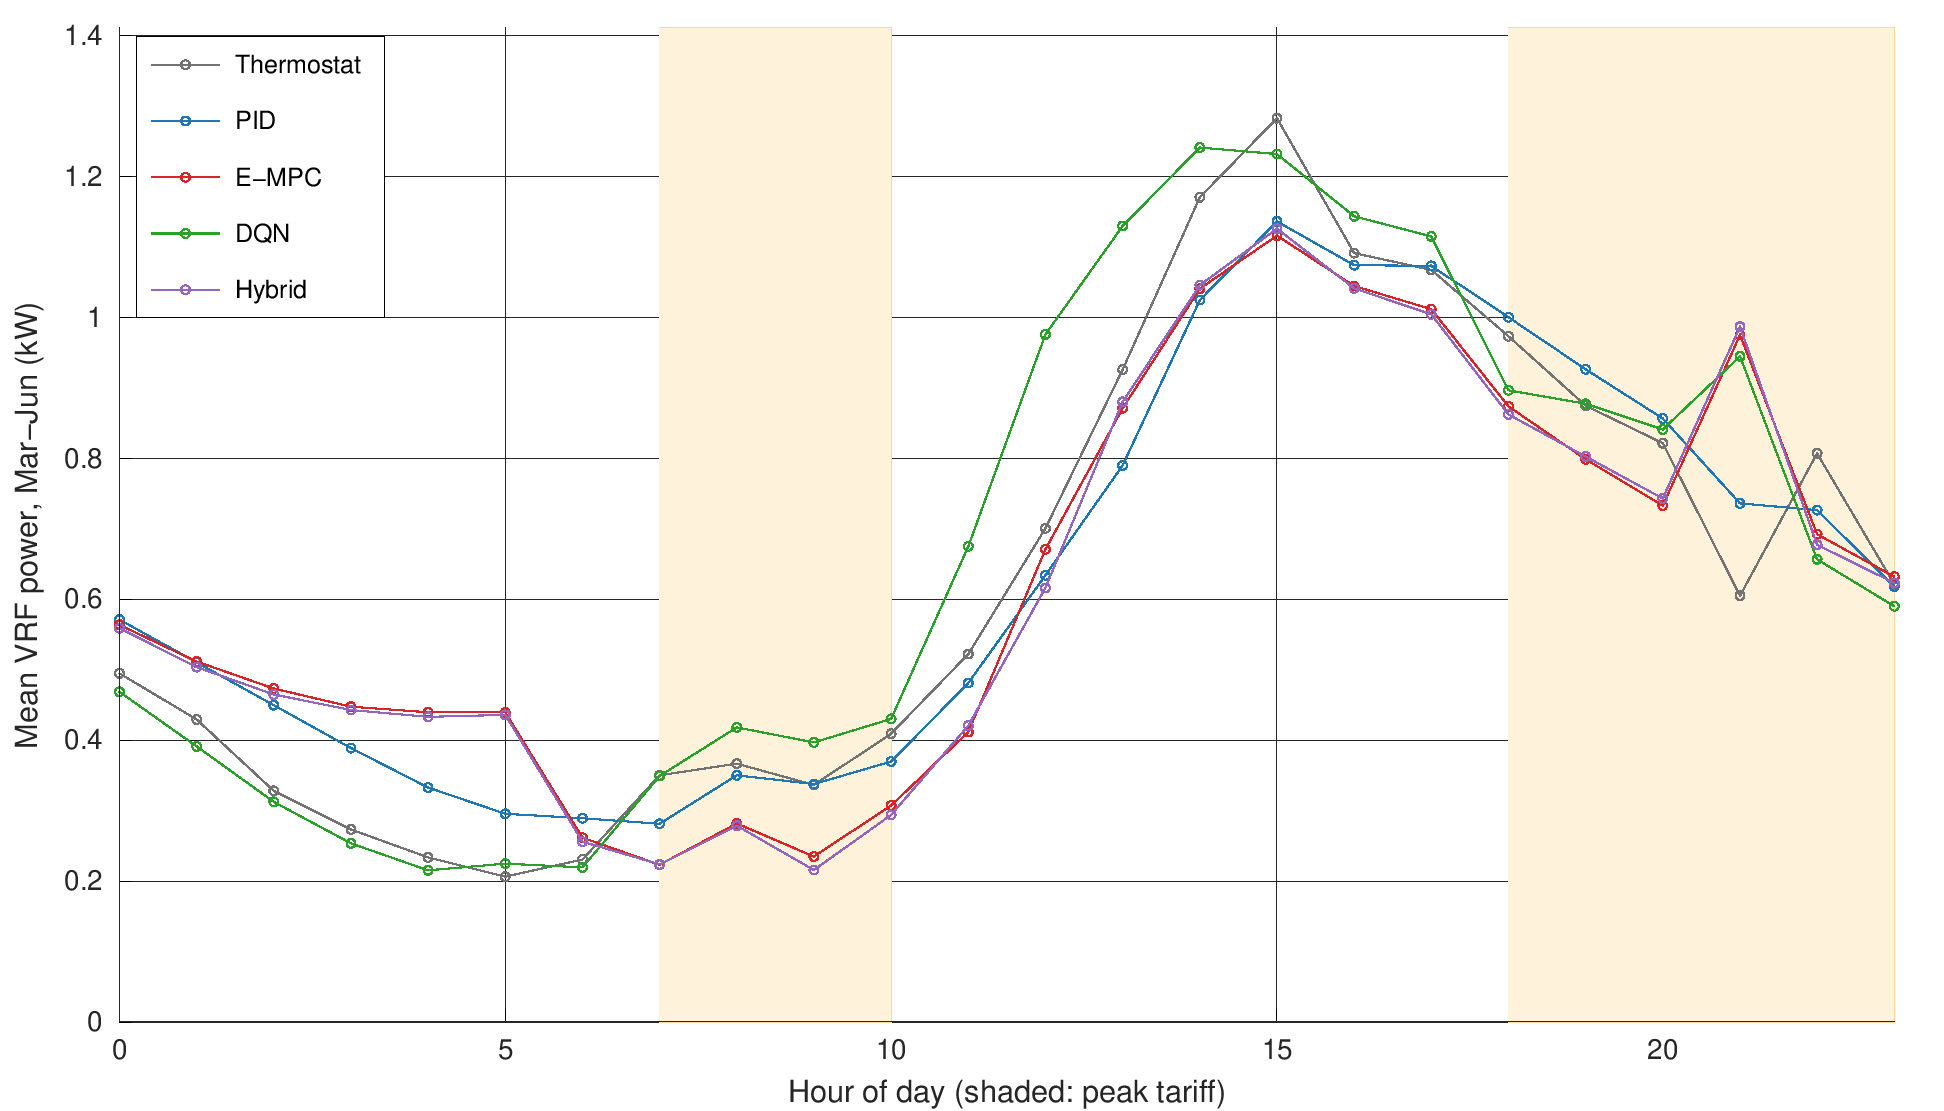
\includegraphics[width=0.7\linewidth]{Fig04_daily_profile.png}
\caption{Mean VRF power by hour of day, March--June, seed 1; peak-tariff hours shaded.}
\label{fig:profile}
\end{figure}

\subsection{Comfort by zone}
Fig.~\ref{fig:comfort}a shows that the ranking holds in every zone. The temperature
distributions in Fig.~\ref{fig:comfort}b show how the controllers differ:
\begin{itemize}
  \item PID concentrates at its 24.5\,$^\circ$C setpoint;
  \item E-MPC and Hybrid concentrate just below 25.5\,$^\circ$C (the band edge minus
        the back-off), which is why they use less energy than PID;
  \item the thermostat and DQN distributions are broad, and the thermostat's has a
        long cold tail.
\end{itemize}

\begin{figure}[t]\centering
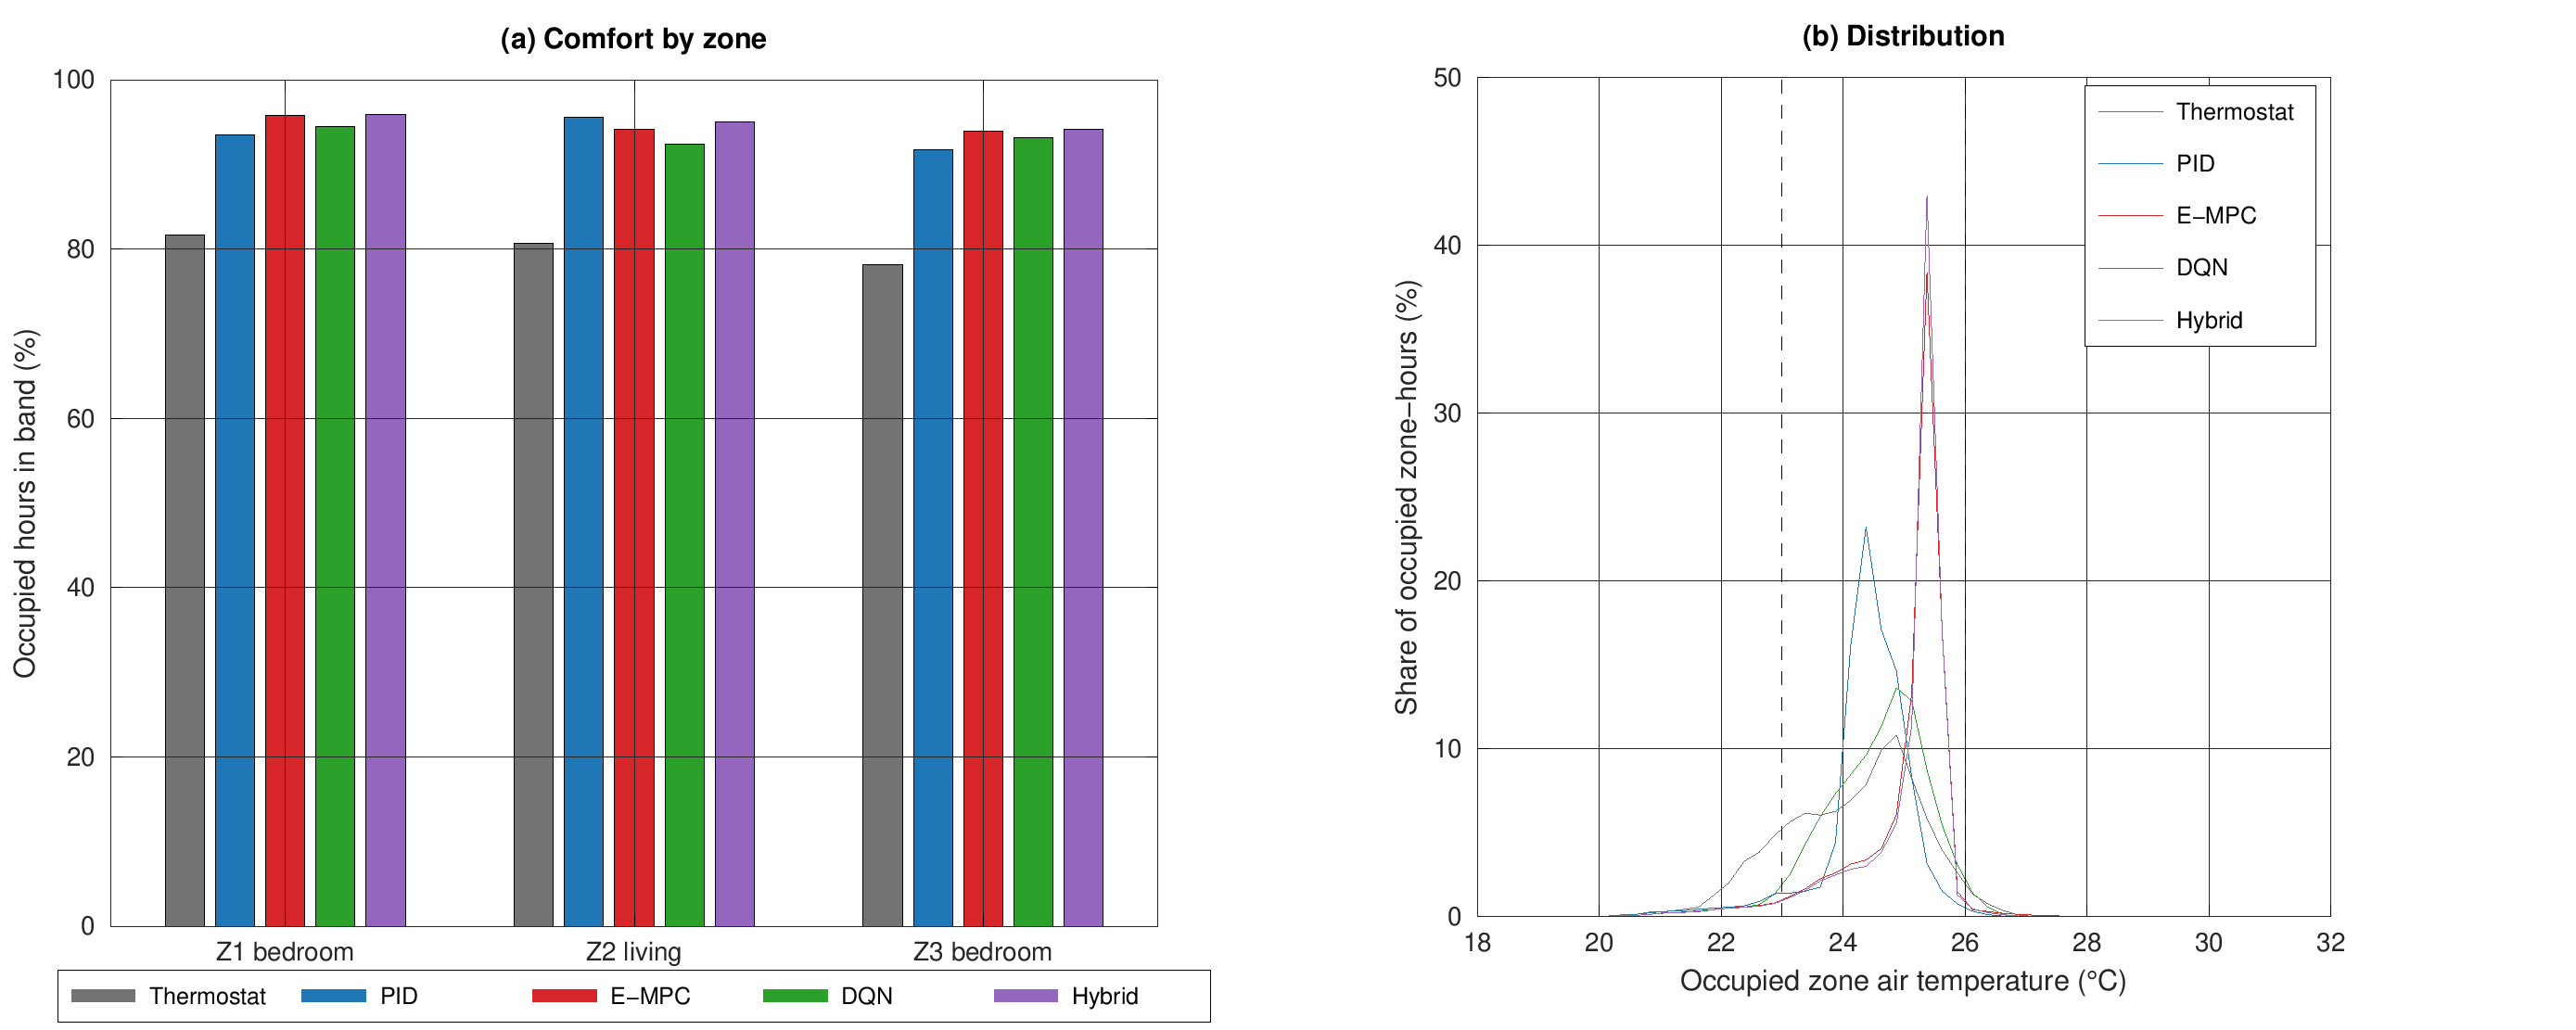
\includegraphics[width=\linewidth]{Fig06_comfort.png}
\caption{(a) Share of occupied hours within the comfort band by zone; (b) distribution of
occupied zone air temperatures (all zones), seed 1.}\label{fig:comfort}
\end{figure}

\subsection{Robustness, sensitivity and ablations}\label{sec:sens}
Table~\ref{tab:sens} and Fig.~\ref{fig:sens} report single-seed results for each
scenario.

\paragraph{Heatwave (+3\,K all year).}
The DQN never saw this weather in training. Cooling cost rises by about a third for all
controllers, and discomfort falls because a warmer winter means less cooling-induced
overcooling. Results:
\begin{itemize}
  \item Hybrid: INR~\SHeatCostHyb, \SHeatKhHyb\,K\,h, still the best on both criteria;
  \item E-MPC: INR~\SHeatCostMpc, \SHeatKhMpc\,K\,h;
  \item PID: INR~\SHeatCostPid, \SHeatKhPid\,K\,h;
  \item DQN: INR~\SHeatCostDqn, \SHeatKhDqn\,K\,h, the most expensive of the
        modulating controllers;
  \item thermostat: \SHeatKhTh\,K\,h.
\end{itemize}
Under sustained heat PID's discomfort falls below E-MPC's. Two tests separate the
possible causes. Giving the E-MPC a perfect model and perfect weather forecasts in the
heatwave year does not help (INR~\SHeatPerfCostMpc, \SHeatPerfKhMpc\,K\,h), so
prediction error is not the cause. Raising the E-MPC back-off from 0.5 to 1.0\,K does
help: discomfort falls to \SHeatBackKhMpc\,K\,h, close to PID's \SHeatKhPid\,K\,h,
at a cost of INR~\SHeatBackCostMpc. The E-MPC loses on comfort because it
deliberately operates close to the upper bound, while PID holds 24.5\,$^\circ$C with
a 1.5\,K margin; under sustained high load, small excursions above a bound that is
barely respected accumulate. With the same 1.0\,K back-off the Hybrid reaches
\SHeatBackKhHyb\,K\,h at INR~\SHeatBackCostHyb. The comfort--cost trade-off is
therefore partly a tuning choice. The shielded DQN transfers to the
hotter year without retraining, but loses its cost advantage over PID.

\paragraph{Thermal mass.}
Halving the effective mass raises discomfort for every controller, because the air
temperature then follows gains more tightly. With half the mass, E-MPC's discomfort
rises to \SMassLoKhMpc\,K\,h and Hybrid's to \SMassLoKhHyb\,K\,h. Doubling the mass
reduces discomfort to \SMassHiKhMpc\ and \SMassHiKhHyb\,K\,h respectively, and lowers
cost. All controllers benefit from more mass; Hybrid remains best on both criteria in
both cases.

\paragraph{Tariff.}
Under a flat tariff, E-MPC uses \SFlatEMpc\,kWh, against \SBaseEMpc\,kWh under ToD. That
near-equality confirms that the ToD term barely changes its decisions in this building:
the savings are efficiency gains, not arbitrage. Two further tariffs test whether this
is a property of the building or of the price signal.
\begin{itemize}
  \item \textbf{Steeper three-tier tariff} (INR 4.00/7.15/14.30 per kWh, a 3.6:1
        peak-to-off-peak ratio): the share of VRF energy in peak hours falls from about
        34\,\% to \SSteepPkShMpc{} (E-MPC) and \SSteepPkShHyb{} (Hybrid), against
        \SSteepPkShPid{} for PID and \SSteepPkShTh{} for the thermostat. A steep enough
        signal does move about 5 percentage points of cooling out of the peak windows.
  \item \textbf{Actual MSEDCL residential structure} (flat INR 7.15 per kWh with a
        INR 0.80 rebate between 09:00 and 17:00): annual costs are INR~\SMsedclCostTh{}
        (thermostat), \SMsedclCostPid{} (PID), \SMsedclCostMpc{} (E-MPC),
        \SMsedclCostDqn{} (DQN) and \SMsedclCostHyb{} (Hybrid), with discomfort
        unchanged from the base case. The Hybrid remains the most comfortable and is
        still 4.4\,\% cheaper than PID, but the DQN is now marginally (0.1\,\%)
        cheaper than the Hybrid. The DQN places 45\,\% of its VRF energy in rebate hours,
        against about 41\,\% for the thermostat, E-MPC and Hybrid; the E-MPC and Hybrid
        do not exploit the small rebate.
\end{itemize}

\paragraph{Information.}
Removing the mismatch changes the plant itself, which then has the nominal, smaller
gains. Costs therefore fall for every controller, including the thermostat
(INR~\SNoMisCostTh). E-MPC falls to INR~\SNoMisCostMpc{} and \SNoMisKhMpc\,K\,h, and
Hybrid to INR~\SNoMisCostHyb{} and \SNoMisKhHyb\,K\,h; the ranking is unchanged. Giving the E-MPC its exact envelope model and perfect weather forecasts
yields INR~\SPerfCostMpc{} and \SPerfKhMpc\,K\,h, no better than the base case. The
remaining gap comes from features the MPC's linear cost does not represent:
\begin{itemize}
  \item VRF part-load and latent behaviour;
  \item IEC and DOAS heat;
  \item the 15-min dynamics inside each hourly block.
\end{itemize}
The Hybrid's feedback layer is designed to correct these. The ablations below show how
much of the Hybrid's advantage the feedback layer actually provides.

\paragraph{Hybrid ablations.}
Removing the PI layer (safety override kept) gives INR~\SNoPICostHyb{} and
\SNoPIKhHyb\,K\,h. Removing the safety override (PI kept) gives INR~\SNoSafeCostHyb{}
and \SNoSafeKhHyb\,K\,h. The full Hybrid gives INR~\SBaseCostHyb{} and
\SBaseKhHyb\,K\,h, and the E-MPC alone INR~\SBaseCostMpc{} and \SBaseKhMpc\,K\,h.
The PI layer therefore provides essentially all of the cost advantage over E-MPC.
Most (about 70\,\%) of the comfort advantage comes from the E-MPC with the safety
override alone. Each layer contributes a little comfort on top of the other.

\paragraph{Uncertainty in assumed inputs.}
Eleven inputs that were assumed rather than measured were varied together in a
\UqN-sample Latin hypercube (single seed):
\begin{itemize}
  \item wall, roof and glazing U-values;
  \item SHGC;
  \item infiltration;
  \item rated COP;
  \item the part-load curve;
  \item occupants;
  \item internal gains;
  \item thermal mass;
  \item the cooking split.
\end{itemize}
Results:
\begin{itemize}
  \item The Hybrid had the lowest discomfort of the modulating controllers in
        \UqBestKhHyb\,\% of samples and the lowest cost in \UqBestCostHyb\,\%
        (the DQN in the rest).
  \item The Hybrid was both cheaper and more comfortable than PID in \UqDomHP\,\% of
        samples, and than E-MPC in \UqDomHM\,\%.
  \item Its cost difference from PID ranged from $\UqHPcostLo$\,\% to
        $\UqHPcostHi$\,\% (5th--95th percentile; median $\UqHPcostMed$\,\%).
  \item Its cost difference from E-MPC was small but consistent: $\UqHMcostLo$\,\% to
        $\UqHMcostHi$\,\%.
  \item The thermostat was cheapest and least comfortable in every sample.
\end{itemize}
The Hybrid's cost advantage over PID shrinks for lighter, more glazed or poorly
insulated roofs (Spearman $\rho$ = 0.60 for roof U-value, 0.49 for SHGC and $-0.38$
for thermal mass). The ranking of the controllers is therefore robust to the assumed
inputs; the size of the saving is not.

\paragraph{MPC horizon.}
Short horizons do slightly better: 6\,h gives INR~\SHorSixCostMpc{} and
\SHorSixKhMpc\,K\,h; 12\,h gives INR~\SHorTwelveCostMpc{} and \SHorTwelveKhMpc\,K\,h;
24\,h gives INR~\SBaseCostMpc{} and \SBaseKhMpc\,K\,h. With forecast errors that grow
with lead time and hourly move blocking, the extra foresight does not pay off.

\paragraph{DQN design.}
\begin{itemize}
  \item Without the safety shield, the agent cools through much of the winter and
        discomfort rises to \SNoShieldKhDqn\,K\,h, at INR~\SNoShieldCostDqn.
  \item With 3 action levels: INR~\SLevThreeCostDqn, \SLevThreeKhDqn\,K\,h.
  \item With 9 action levels: INR~\SLevNineCostDqn, \SLevNineKhDqn\,K\,h.
\end{itemize}

\begin{figure}[t]\centering
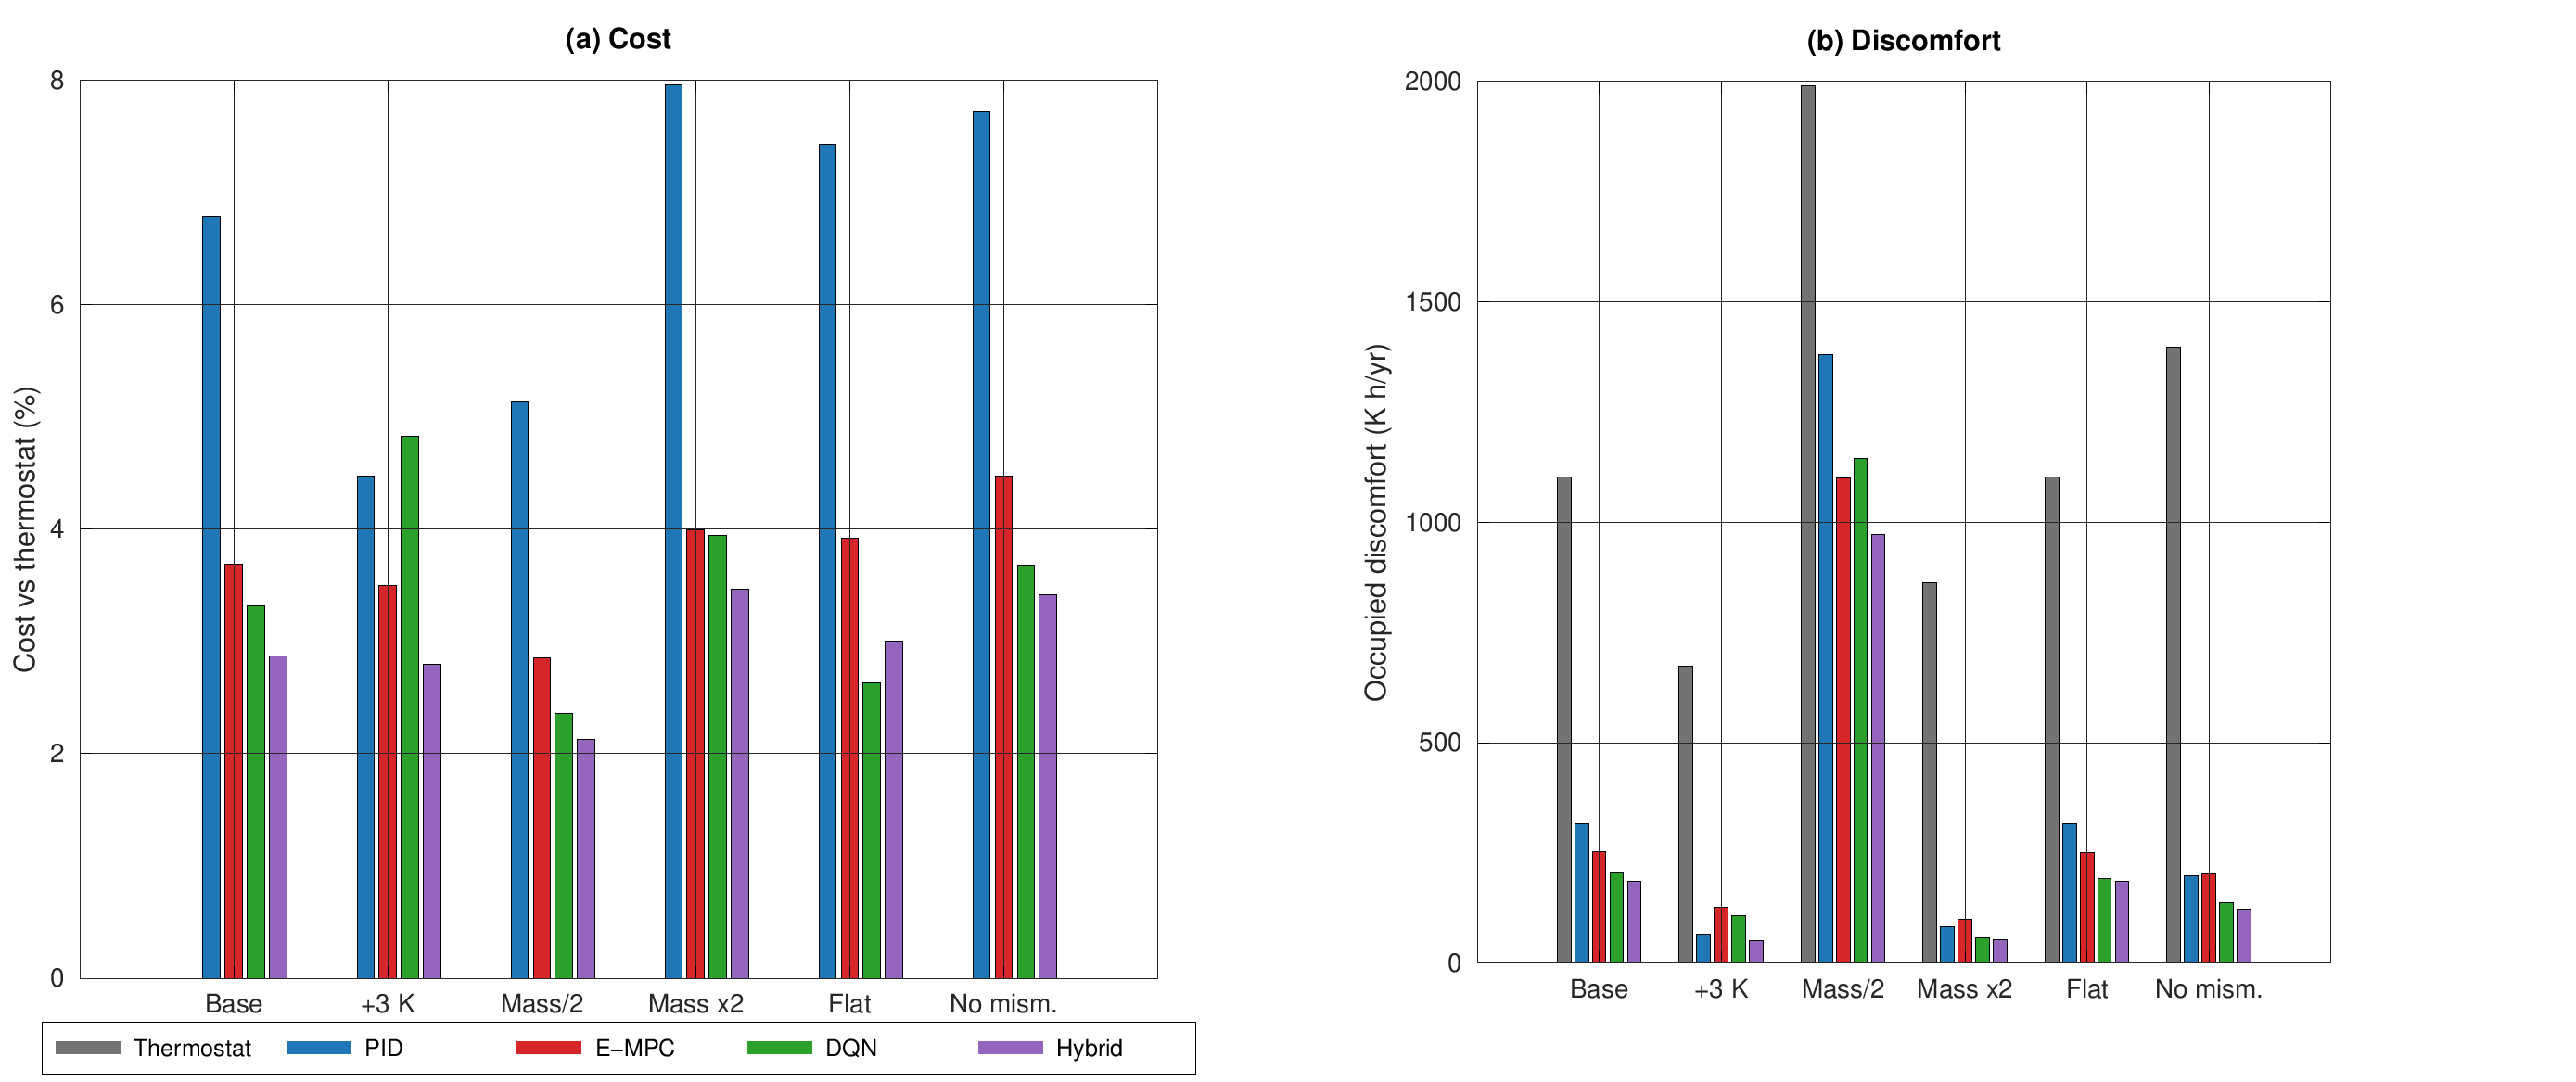
\includegraphics[width=\linewidth]{Fig08_sensitivity.png}
\caption{Sensitivity of (a) annual cost relative to the thermostat and (b) occupied
discomfort across scenarios (seed 1).}\label{fig:sens}
\end{figure}

\subsection{Indoor air quality and ventilation architecture}
CO$_2$ and PM$_{2.5}$ depend on the ventilation and filtration design, not on the
thermal controller (Fig.~\ref{fig:iaq}). Humidity depends on both: controllers that
cool more steadily also remove more moisture.
\begin{itemize}
  \item \textbf{Base design} (continuous 28\,L\,s$^{-1}$ DOAS with MERV-13 filtration
        plus HEPA recirculation), Hybrid controller: mean CO$_2$ \SBaseCoHyb\,ppm; mean
        indoor PM$_{2.5}$ \SBasePmHyb\,$\mu$g\,m$^{-3}$, below the outdoor annual mean
        of about 33\,$\mu$g\,m$^{-3}$; no day above the Indian NAAQS 24-h limit; and
        \SBasePmDHyb\ days above the WHO 24-h guideline, driven by cooking and winter
        outdoor pollution.
  \item \textbf{No recirculation filter}: mean PM$_{2.5}$ rises to
        \SNoFiltPmHyb\,$\mu$g\,m$^{-3}$, above the WHO guideline on every day.
  \item \textbf{CO$_2$}: in the well-mixed whole-dwelling balance it never exceeds
        1000\,ppm in any scenario. Even without mechanical ventilation, 0.5\,ACH of
        infiltration bounds it at about 970\,ppm, against a mean of \SBaseCoHyb\,ppm
        with the DOAS. This is a limitation of the single-volume IAQ model: closed
        bedrooms at night would reach higher concentrations.
  \item \textbf{Humidity}: here the DOAS matters most. Occupied hours with indoor RH
        above 70\,\% are \SVentOffRhHyb\ with no mechanical ventilation, \SVentHumRhHyb\
        with the original humidity-triggered DOAS (60\,L\,s$^{-1}$ in humid weather only),
        and \SBaseRhHyb\ with the demand-controlled dehumidifying DOAS. The original
        design also uses more DOAS energy.
\end{itemize}
The original study reported 160--195\,$\mu$g\,m$^{-3}$ of indoor PM$_{2.5}$ despite HEPA
filtration. That result came from an unstable explicit integration of the mass balance.
With exact integration, recirculating HEPA filtration keeps indoor PM$_{2.5}$ well below
outdoor levels.

\begin{figure}[t]\centering
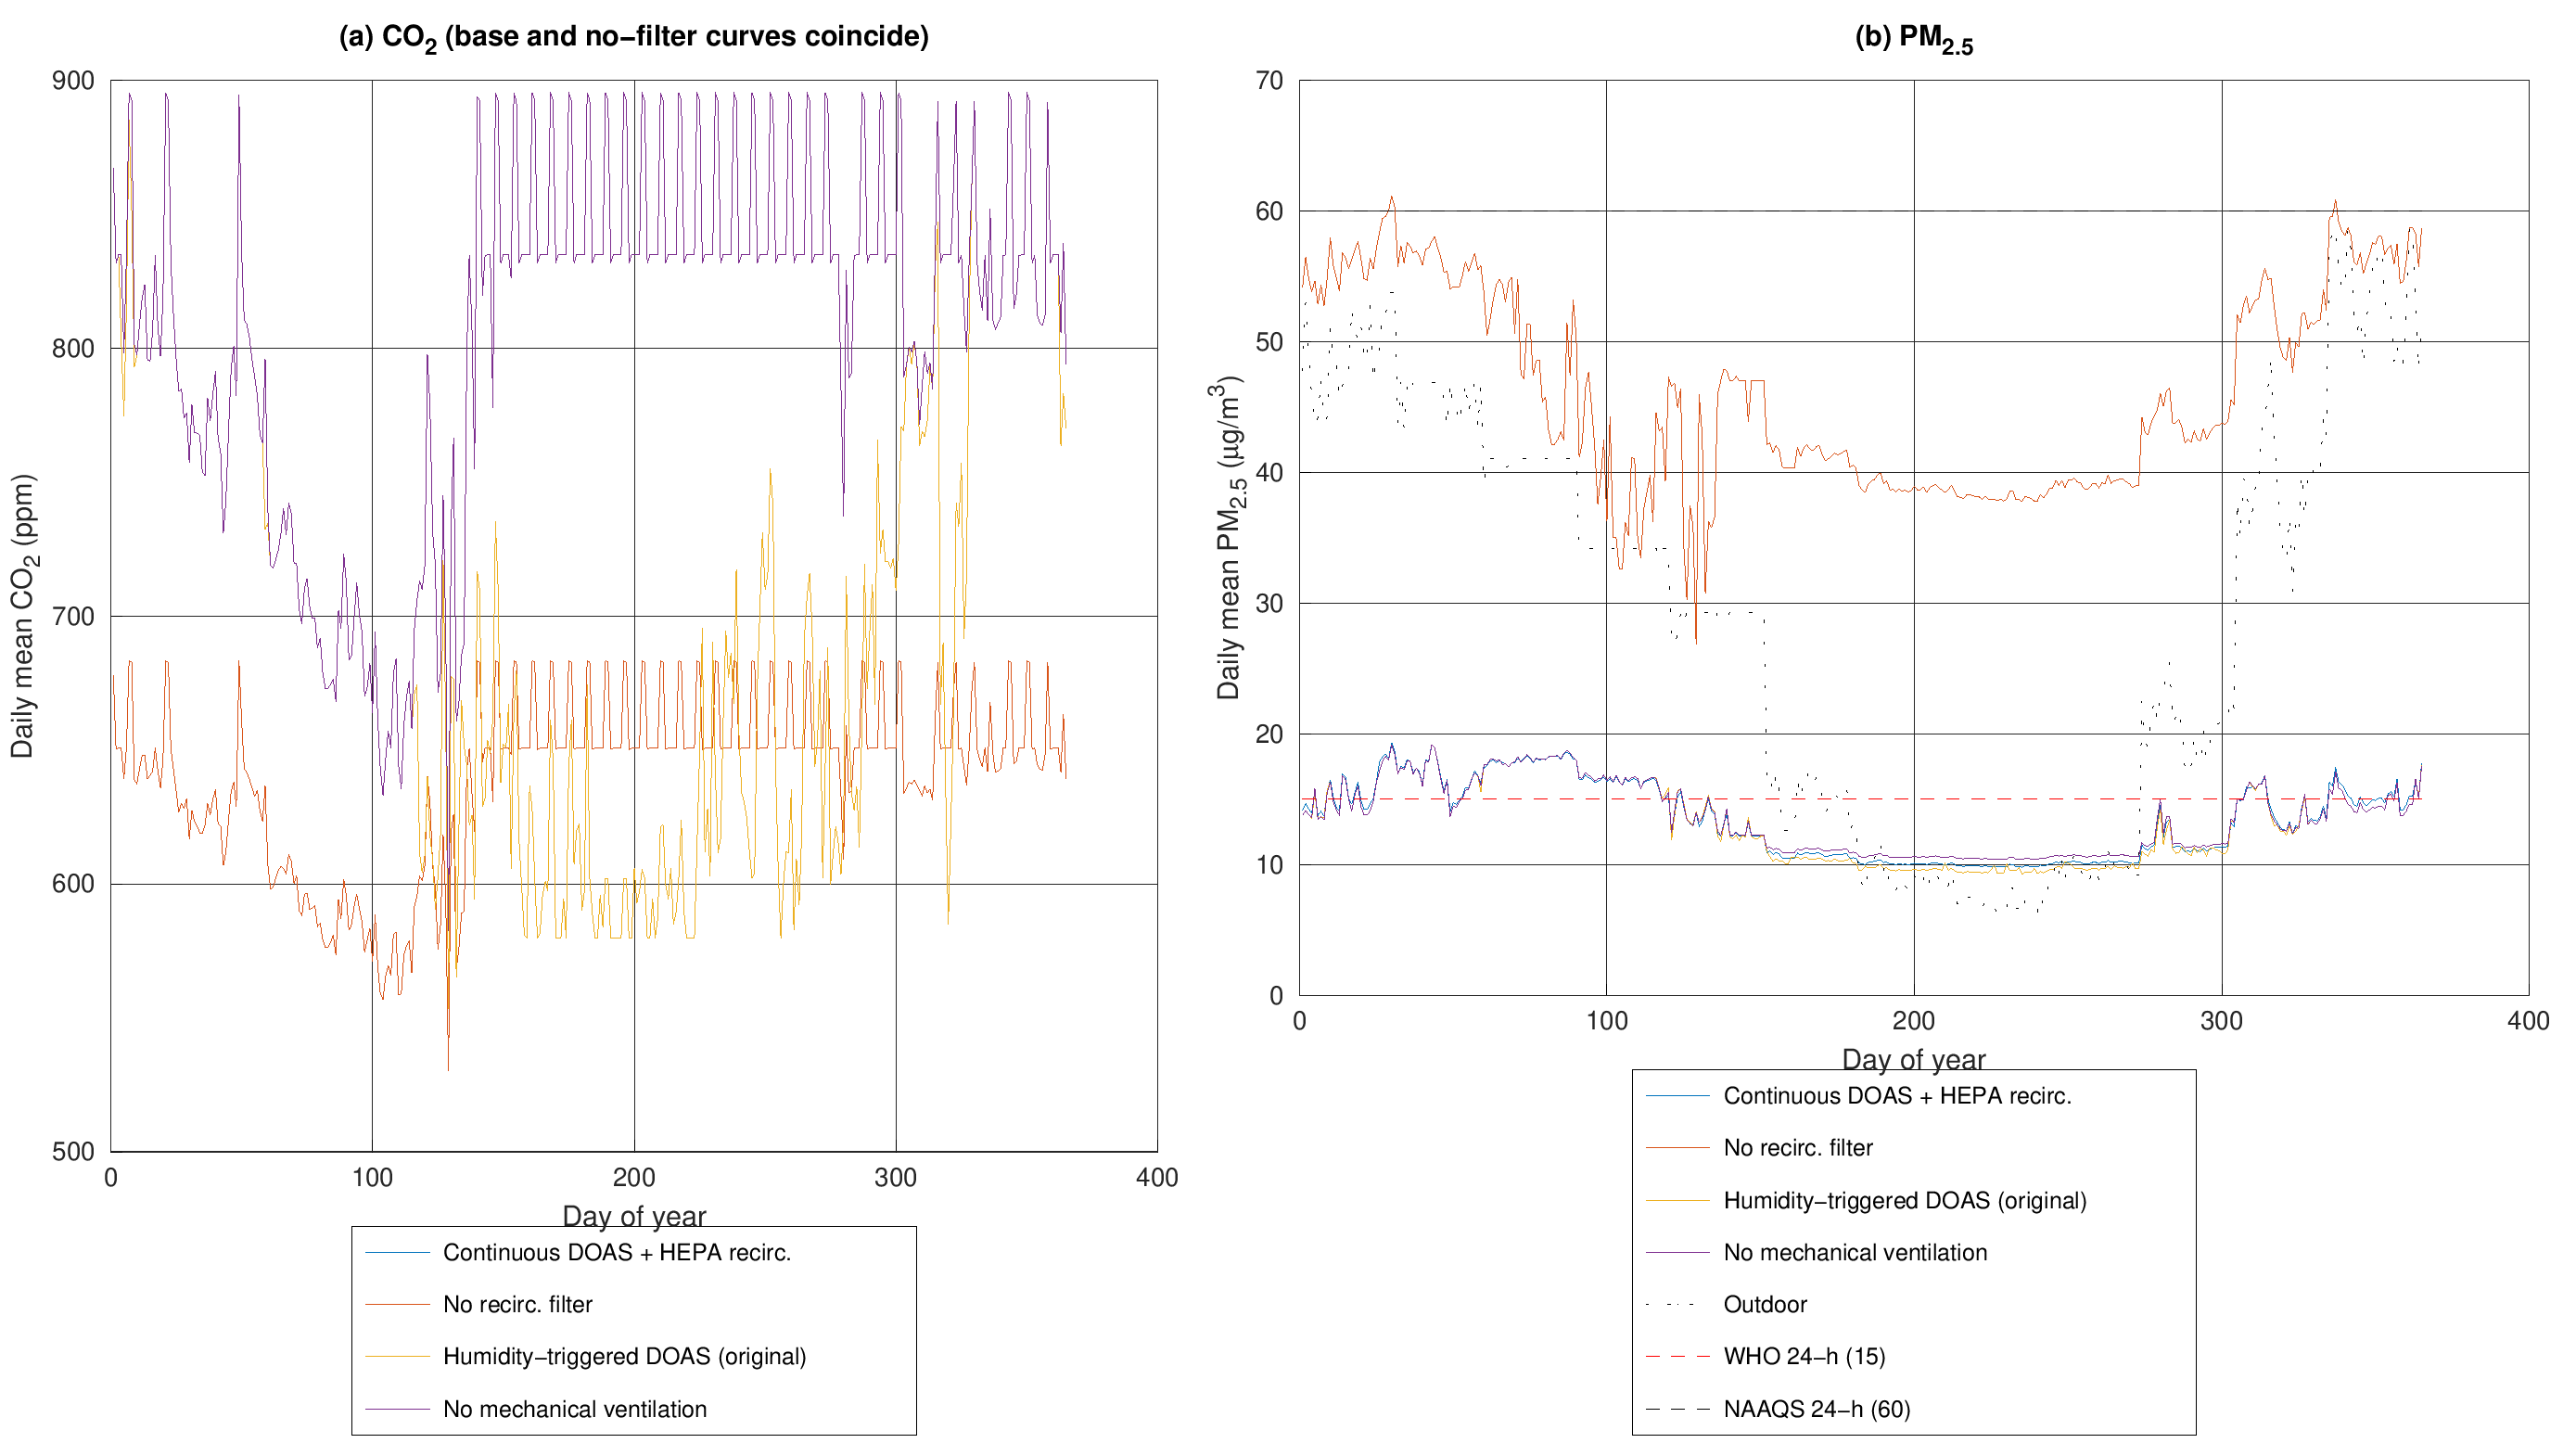
\includegraphics[width=\linewidth]{Fig07_iaq.png}
\caption{Daily mean indoor CO$_2$ (a) and PM$_{2.5}$ (b) for four ventilation/filtration
architectures (Hybrid controller).}\label{fig:iaq}
\end{figure}

\begin{table}[t]\centering\small
\caption{Selected sensitivity and ablation results (seed 1). Cost in INR, discomfort in K\,h.}\label{tab:sens}
\begin{tabular}{lrrrrrrrr}\toprule
 & \multicolumn{2}{c}{PID} & \multicolumn{2}{c}{E-MPC} & \multicolumn{2}{c}{DQN} & \multicolumn{2}{c}{Hybrid}\\
Scenario & Cost & K\,h & Cost & K\,h & Cost & K\,h & Cost & K\,h\\\midrule
Base & \SBaseCostPid & \SBaseKhPid & \SBaseCostMpc & \SBaseKhMpc & \SBaseCostDqn & \SBaseKhDqn & \SBaseCostHyb & \SBaseKhHyb\\
Heatwave +3\,K & \SHeatCostPid & \SHeatKhPid & \SHeatCostMpc & \SHeatKhMpc & \SHeatCostDqn & \SHeatKhDqn & \SHeatCostHyb & \SHeatKhHyb\\
Mass $\times$0.5 & \SMassLoCostPid & \SMassLoKhPid & \SMassLoCostMpc & \SMassLoKhMpc & \SMassLoCostDqn & \SMassLoKhDqn & \SMassLoCostHyb & \SMassLoKhHyb\\
Mass $\times$2 & \SMassHiCostPid & \SMassHiKhPid & \SMassHiCostMpc & \SMassHiKhMpc & \SMassHiCostDqn & \SMassHiKhDqn & \SMassHiCostHyb & \SMassHiKhHyb\\
Flat tariff & \SFlatCostPid & \SFlatKhPid & \SFlatCostMpc & \SFlatKhMpc & \SFlatCostDqn & \SFlatKhDqn & \SFlatCostHyb & \SFlatKhHyb\\
No mismatch & \SNoMisCostPid & \SNoMisKhPid & \SNoMisCostMpc & \SNoMisKhMpc & \SNoMisCostDqn & \SNoMisKhDqn & \SNoMisCostHyb & \SNoMisKhHyb\\
Perfect info & -- & -- & \SPerfCostMpc & \SPerfKhMpc & -- & -- & \SPerfCostHyb & \SPerfKhHyb\\
Horizon 6\,h & -- & -- & \SHorSixCostMpc & \SHorSixKhMpc & -- & -- & \SHorSixCostHyb & \SHorSixKhHyb\\
Horizon 12\,h & -- & -- & \SHorTwelveCostMpc & \SHorTwelveKhMpc & -- & -- & \SHorTwelveCostHyb & \SHorTwelveKhHyb\\
\bottomrule\end{tabular}
\end{table}

